\documentclass{ximera}
\graphicspath{  %% When looking for images,
{./}            %% look here first,
{./pictures/}   %% then look for a pictures folder,
{../pictures/}  %% which may be a directory up.
{../../pictures/}  %% which may be a directory up.
{../../../pictures/}  %% which may be a directory up.
{../../../../pictures/}  %% which may be a directory up.
}

\usepackage{listings}
\usepackage{circuitikz}
\usepackage{xcolor}
\usepackage{amsmath,amsthm}
\usepackage{subcaption}
\usepackage{graphicx}
\usepackage{tikz}
\usepackage{tikz-3dplot}
\usepackage{amsfonts}
\usepackage{mdframed} % For framing content
\usepackage{tikz-cd}

  \renewcommand{\vector}[1]{\left\langle #1\right\rangle}
  \newcommand{\arrowvec}[1]{{\overset{\rightharpoonup}{#1}}}
  \newcommand{\ro}{\texttt{R}}%% row operation
  \newcommand{\dotp}{\bullet}%% dot product
  \renewcommand{\l}{\ell}
  \let\defaultAnswerFormat\answerFormatBoxed
  \usetikzlibrary{calc,bending}
  \tikzset{>=stealth}
  




%make a maroon color
\definecolor{maroon}{RGB}{128,0,0}
%make a dark blue color
\definecolor{darkblue}{RGB}{0,0,139}
%define the color fourier0 to be the maroon color
\definecolor{fourier0}{RGB}{128,0,0}
%define the color fourier1 to be the dark blue color
\definecolor{fourier1}{RGB}{0,0,139}
%define the color fourier 1t to be the light blue color
\definecolor{fourier1t}{RGB}{173,216,230}
%define the color fourier2 to be the dark green color
\definecolor{fourier2}{RGB}{0,100,0}
%define teh color fourier2t to be the light green color
\definecolor{fourier2t}{RGB}{144,238,144}
%define the color fourier3 to be the dark purple color
\definecolor{fourier3}{RGB}{128,0,128}
%define the color fourier3t to be the light purple color
\definecolor{fourier3t}{RGB}{221,160,221}
%define the color fourier0t to be the red color
\definecolor{fourier0t}{RGB}{255,0,0}
%define the color fourier4 to be the orange color
\definecolor{fourier4}{RGB}{255,165,0}
%define the color fourier4t to be the darker orange color
\definecolor{fourier4t}{RGB}{255,215,0}
%define the color fourier5 to be the yellow color
\definecolor{fourier5}{RGB}{255,255,0}
%define the color fourier5t to be the darker yellow color
\definecolor{fourier5t}{RGB}{255,255,100}
%define the color fourier6 to be the green color
\definecolor{fourier6}{RGB}{0,128,0}
%define the color fourier6t to be the darker green color
\definecolor{fourier6t}{RGB}{0,255,0}

%New commands for this doc for errors in copying
\newcommand{\eigenvar}{\lambda}
%\newcommand{\vect}[1]{\mathbf{#1}}
\renewcommand{\th}{^{\text{th}}}
\newcommand{\st}{^{\text{st}}}
\newcommand{\nd}{^{\text{nd}}}
\newcommand{\rd}{^{\text{rd}}}
\newcommand{\paren}[1]{\left(#1\right)}
\newcommand{\abs}[1]{\left|#1\right|}
\newcommand{\R}{\mathbb{R}}
\newcommand{\C}{\mathbb{C}}
\newcommand{\Hilb}{\mathbb{H}}
\newcommand{\qq}[1]{\text{#1}}
\newcommand{\Z}{\mathbb{Z}}
\newcommand{\N}{\mathbb{N}}
\newcommand{\q}[1]{\text{``#1''}}
%\newcommand{\mat}[1]{\begin{bmatrix}#1\end{bmatrix}}
\newcommand{\rref}{\text{reduced row echelon form}}
\newcommand{\ef}{\text{echelon form}}
\newcommand{\ohm}{\Omega}
\newcommand{\volt}{\text{V}}
\newcommand{\amp}{\text{A}}
\newcommand{\Seq}{\textbf{Seq}}
\newcommand{\Poly}{\textbf{P}}
\renewcommand{\quad}{\text{    }}
\newcommand{\roweq}{\simeq}
\newcommand{\rowop}{\simeq}
\newcommand{\rowswap}{\leftrightarrow}
\newcommand{\Mat}{\textbf{M}}
\newcommand{\Func}{\textbf{Func}}
\newcommand{\Hw}{\textbf{Hamming weight}}
\newcommand{\Hd}{\textbf{Hamming distance}}
\newcommand{\rank}{\text{rank}}
\newcommand{\longvect}[1]{\overrightarrow{#1}}
% Define the circled command
\newcommand{\circled}[1]{%
  \tikz[baseline=(char.base)]{
    \node[shape=circle,draw,inner sep=2pt,red,fill=red!20,text=black] (char) {#1};}%
}

% Define custom command \strikeh that just puts red text on the 2nd argument
\newcommand{\strikeh}[2]{\textcolor{red}{#2}}

% Define custom command \strikev that just puts red text on the 2nd argument
\newcommand{\strikev}[2]{\textcolor{red}{#2}}

%more new commands for this doc for errors in copying
\newcommand{\SI}{\text{SI}}
\newcommand{\kg}{\text{kg}}
\newcommand{\m}{\text{m}}
\newcommand{\s}{\text{s}}
\newcommand{\norm}[1]{\left\|#1\right\|}
\newcommand{\col}{\text{col}}
\newcommand{\sspan}{\text{span}}
\newcommand{\proj}{\text{proj}}
\newcommand{\set}[1]{\left\{#1\right\}}
\newcommand{\degC}{^\circ\text{C}}
\newcommand{\centroid}[1]{\overline{#1}}
\newcommand{\dotprod}{\boldsymbol{\cdot}}
%\newcommand{\coord}[1]{\begin{bmatrix}#1\end{bmatrix}}
\newcommand{\iprod}[1]{\langle #1 \rangle}
\newcommand{\adjoint}{^{*}}
\newcommand{\conjugate}[1]{\overline{#1}}
\newcommand{\eigenvarA}{\lambda}
\newcommand{\eigenvarB}{\mu}
\newcommand{\orth}{\perp}
\newcommand{\bigbracket}[1]{\left[#1\right]}
\newcommand{\textiff}{\text{ if and only if }}
\newcommand{\adj}{\text{adj}}
\newcommand{\ijth}{\emph{ij}^\text{th}}
\newcommand{\minor}[2]{M_{#2}}
\newcommand{\cofactor}{\text{C}}
\newcommand{\shift}{\textbf{shift}}
\newcommand{\startmat}[1]{
  \left[\begin{array}{#1}
}
\newcommand{\stopmat}{\end{array}\right]}
%a command to give a name to explorations and hints and theorems
\newcommand{\name}[1]{\begin{centering}\textbf{#1}\end{centering}}
\newcommand{\vect}[1]{\vec{#1}}
\newcommand{\dfn}[1]{\textbf{#1}}
\newcommand{\transpose}{\mathsf{T}}
\newcommand{\mtlb}[2][black]{\texttt{\textcolor{#1}{#2}}}
\newcommand{\RR}{\mathbb{R}} % Real numbers
\newcommand{\id}{\text{id}}

\author{Zack Reed}
%borrowed from selinger linear algebra
\title{Learning Activity: }
\begin{document}
\begin{abstract}

    In this learning activity, you will be 
\end{abstract}
\maketitle
 
\section*{Composition and Inverses of Linear Transformations}
 
\subsection*{Composition of Linear Transformations}
\begin{definition}\label{def:compoflintrans} Let $U$, $V$ and $W$ be vector spaces, and let $T:U\rightarrow V$ and $S:V\rightarrow W$ be linear transformations.  The \dfn{composition} of $S$ and $T$ is the transformation $S\circ T:U\rightarrow W$ given by
$$(S\circ T)(\vec{u})=S(T(\vec{u}))$$
\end{definition}
 
\begin{example}\label{ex:transcomp} Define $$T:\RR^2\rightarrow \RR^2 \quad\text{by}\quad T\left(\begin{bmatrix}u_1\\u_2\end{bmatrix}\right)=\begin{bmatrix}u_1+u_2\\3u_1+3u_2\end{bmatrix}$$
 
$$S:\RR^2\rightarrow \RR^2 \quad\text{by}\quad S\left(\begin{bmatrix}v_1\\v_2\end{bmatrix}\right)=\begin{bmatrix}3v_1-v_2\\-3v_1+v_2\end{bmatrix}$$
(You should be able to verify that both transformations are linear.)  Examine the effect of $S\circ T$ on vectors of $\RR^2$.
\begin{explanation}
From the computational standpoint, the situation is simple.
\begin{align*}
(S\circ T)\left(\begin{bmatrix}u_1\\u_2\end{bmatrix}\right)&=S\left(T\left(\begin{bmatrix}u_1\\u_2\end{bmatrix}\right)\right)=S\left(\begin{bmatrix}u_1+u_2\\3u_1+3u_2\end{bmatrix}\right)\\
&=\begin{bmatrix}3(u_1+u_2)-(3u_1+3u_2)\\-3(u_1+u_2)+(3u_1+3u_2)\end{bmatrix}\\
&=\vec{0}
\end{align*}
This means that $S\circ T$ maps all vectors of $\RR^2$ to $\vec{0}$. 
 
In addition to the computational approach, it is also useful to visualize what happens geometrically.
 
First, observe that $$T\left(\begin{bmatrix}u_1\\u_2\end{bmatrix}\right)=\begin{bmatrix}u_1+u_2\\3u_1+3u_2\end{bmatrix}=(u_1+u_2)\begin{bmatrix}1\\3\end{bmatrix}$$  Therefore the image of any vector of $\RR^2$ under $T$ lies on the line determined by the vector $\begin{bmatrix}1\\3\end{bmatrix}$. 
 
Even though $S$ is defined on all of $\RR^2$, we are only interested in the action of $S$ on vectors along the line determined by $\begin{bmatrix}1\\3\end{bmatrix}$.  Our computations showed that all such vectors map to $\vec{0}$.
 
The actions of individual transformations, as well as the composite transformation are shown below.
 
\begin{center}
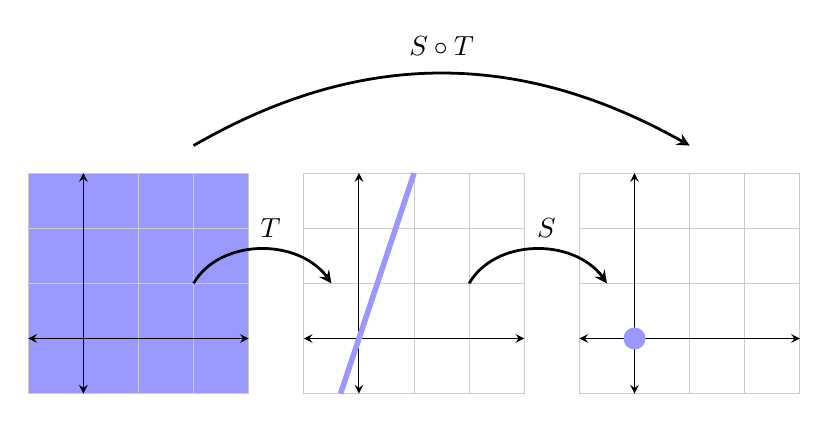
\begin{tikzpicture}[scale=0.7]
 
\fill[blue!40] (-1,-1) rectangle (3,3);
\draw[thin,gray!40] (-1,-1) grid (3,3);
  \draw[<->] (-1,0)--(3,0);
  \draw[<->] (0,-1)--(0,3);
 
  \draw[thin,gray!40] (4,-1) grid (8,3);
  \draw[<->] (4,0)--(8,0);
  \draw[<->] (5,-1)--(5,3);
  \draw[line width=2pt,blue!40](14/3,-1)--(6,3) node[anchor=south west]{};
   
  \draw[thin,gray!40] (9,-1) grid (13,3);
  \draw[<->] (9,0)--(13,0);
  \draw[<->] (10,-1)--(10,3);
   
  \fill[blue!40!white] (10,0) circle (0.2cm);
  \draw [->,line width=1pt,-stealth]  (2,1)to[out=60, in=120](4.5, 1);
   \node[] at (3.4, 2)   (b) {$T$};
\draw [->,line width=1pt,-stealth] (7,1)to[out=60, in=120](9.5, 1);
\node[] at (8.4, 2)   (b) {$S$};
\draw [->,line width=1pt,-stealth] (2,3.5)to[out=30, in=150](11, 3.5);
\node[] at (6.5, 5.3)   (b) {$S\circ T$};
\end{tikzpicture}
\end{center}
 
\end{explanation}
\end{example}
 
\begin{theorem}\label{th:complinear}
The composition of two linear transformations is linear.
\end{theorem}
\begin{proof}
Let $T:U\rightarrow V$ and $S:V\rightarrow W$ be linear transformations. We will show that $S\circ T$ is linear.  For all vectors $\vec{u}_1$ and $\vec{u}_2$ of $U$ and scalars $a$ and $b$ we have:
\begin{align*}
(S\circ T)(a\vec{u}_1+b\vec{u}_2)&=S(T(a\vec{u}_1+b\vec{u}_2))\\
&=S(aT(\vec{u}_1)+bT(\vec{u}_2))\\
&=aS(T(\vec{u}_1))+bS(T(\vec{u}_2))\\
&=a(S\circ T)(\vec{u}_1)+b(S\circ T)(\vec{u}_2)
\end{align*}
\end{proof}

 
\begin{theorem}\label{th:compoflintransass} Composition of linear transformations is associative.  In other words, for linear transformations  $T$, $S$ and $R$


 
    \begin{center}
        \begin{tikzpicture}
        %\node{
        \begin{tikzcd}
        U\rar{T}\arrow[black, bend right]{rrr}[black,swap]{R\circ S\circ T}  & V \rar{S}  & W \rar{R} & Z
        \end{tikzcd}
        %};
        \end{tikzpicture}
    \end{center}
 
We have $(R\circ S)\circ T=R\circ (S\circ T)$.
\end{theorem}



\begin{proof} For all $\vec{u}$ in $U$ we have:
\begin{align*}
((R\circ S)\circ T)(\vec{u})&=(R\circ S)(T(\vec{u}))=R(S(T(\vec{u})))\\
&=R((S\circ T)(\vec{u}))=(R\circ (S\circ T))(\vec{u})
\end{align*}
\end{proof}
 
\subsection*{Composition and Matrix Multiplication}
 
In this section we will consider linear transformations of $\RR^n$ and their standard matrices. 
 
\begin{theorem}\label{th:standardmatcompoflintrans}
Let $T:\RR^n\rightarrow \RR^m$ and $S:\RR^m\rightarrow \RR^p$ be linear transformations with standard matrices $M_T$ and $M_S$, respectively.  Then the composite transformation $S\circ T:\RR^n\rightarrow \RR^p$ has a standard matrix given by the product $M_SM_T$.
\end{theorem}
\begin{proof}
For all $\vec{v}$ in $\RR^n$ we have:
$$(S\circ T)(\vec{v})=S(T(\vec{v}))=S(M_T\vec{v})=M_S(M_T\vec{v})=(M_SM_T)\vec{v}$$
\end{proof}

 
\begin{example}\label{ex:standardmatofcomp}
In Example \ref{ex:transcomp}, we discussed a composite transformation $S\circ T:\RR^2\rightarrow \RR^2$
given by:
$$T\left(\begin{bmatrix}u_1\\u_2\end{bmatrix}\right)=\begin{bmatrix}u_1+u_2\\3u_1+3u_2\end{bmatrix}\quad \text{and} \quad
S\left(\begin{bmatrix}v_1\\v_2\end{bmatrix}\right)=\begin{bmatrix}3v_1-v_2\\-3v_1+v_2\end{bmatrix}$$
Express $S\circ T$ as a matrix transformation.
\begin{explanation}
The standard matrix for $T:\RR^2\rightarrow \RR^2$ is $$\begin{bmatrix}1&1\\3&3\end{bmatrix}$$ and the standard matrix for $S:\RR^2\rightarrow \RR^2$ is $$\begin{bmatrix}3&-1\\-3&1\end{bmatrix}$$
The standard matrix for $S\circ T$ is the product
$$\begin{bmatrix}3&-1\\-3&1\end{bmatrix}\begin{bmatrix}1&1\\3&3\end{bmatrix}=\begin{bmatrix}0&0\\0&0\end{bmatrix}$$
\end{explanation}
\end{example}

 
We conclude this section by revisiting the associative property of matrix multiplication.  At the time matrix multiplication was introduced, we skipped the cumbersome proof that for appropriately sized matrices $A$, $B$ and $C$, we have $(AB)C=A(BC)$. (See Theorem \ref{th:propertiesofmatrixmultiplication}.)  We are now in a position to prove this result with ease. 
 
Every matrix induces a linear transformation.  The product of two matrices can be interpreted as a composition of transformations.  Since function composition is associative, so is matrix multiplication. We formalize this observation as a theorem.
 
\begin{theorem}[Associativity of Matrix Multiplication] \label{th:associativematrixmult}  Let $A$, $B$ and $C$ be matrices of appropriate dimensions so that the product $(AB)C$ is defined.  Then
$$(AB)C=A(BC)$$
\end{theorem}

 
\subsection*{Inverses of Linear Transformations}

 
\begin{exploration}\label{ep:inverse} Define a linear transformation $T:\RR^2\rightarrow \RR^2$ by $T(\vec{v})=2\vec{v}$.  In other words, $T$ doubles every vector in $\RR^2$.  Now define $S:\RR^2\rightarrow \RR^2$ by $S(\vec{v})=\frac{1}{2}\vec{v}$.  What happens when we compose these two transformations?

$$(S\circ T)(\vec{v})=S(T(\vec{v}))=S(2\vec{v})=\left(\frac{1}{2}\right)(2)\vec{v}=\vec{v}$$

$$(T\circ S)(\vec{v})=T(S(\vec{v}))=T(\frac{1}{2}\vec{v})=(2)\left(\frac{1}{2}\right)\vec{v}=\vec{v}$$
Both composite transformations return the original vector $\vec{v}$. 

In other words, $S\circ T$ and $T\circ S$ are just the identity maps.  We say that $S$ is an \dfn{inverse} of $T$, and $T$ is an inverse of $S$.
\end{exploration}



 
\begin{definition}\label{def:inverseoflintrans} Let $V$ and $W$ be vector spaces, and let $T:V\rightarrow W$ be a linear transformation.  A transformation $S:W\rightarrow V$ that satisfies $S\circ T=\id_V$ and $T\circ S=\id_W$ is called an \dfn{inverse} of $T$. If $T$ has an inverse, $T$ is called \dfn{invertible}.
\end{definition}
 
\begin{example}\label{ex:inverseverify} Let $T:\RR^2\rightarrow \RR^2$ be a transformation defined by $T\left(\begin{bmatrix}x\\y\end{bmatrix}\right)=\begin{bmatrix}x+y\\x-y\end{bmatrix}$. (How would you verify that $T$ is linear?)  Show that $S:\RR^2\rightarrow \RR^2$ given by $S\left(\begin{bmatrix}x\\y\end{bmatrix}\right)=\begin{bmatrix}0.5x+0.5y\\0.5x-0.5y\end{bmatrix}$ is an inverse of $T$.
\begin{explanation}
We will show that $S\circ T=\id_{\RR^2}$. 
\begin{align*}
(S\circ T)\left(\begin{bmatrix}x\\y\end{bmatrix}\right)&=S\left(T\left(\begin{bmatrix}x\\y\end{bmatrix}\right)\right)=S\left(\begin{bmatrix}x+y\\x-y\end{bmatrix}\right)\\
&=\begin{bmatrix}0.5(x+y)+0.5(x-y)\\0.5(x+y)-0.5(x-y)\end{bmatrix}
=\begin{bmatrix}x\\y\end{bmatrix}
\end{align*}
We leave it to the reader to verify that $T\circ S=\id_{\RR^2}$.
 
\end{explanation}
\end{example}

 
\subsection*{Linearity of Inverses of Linear Transformations}
 
Definition \ref{def:inverseoflintrans} does not specifically require an inverse $S$ of a linear transformation $T$ to be linear, but it turns out that the requirement that $S\circ T=\id_V$ and $T\circ S=\id_W$ is sufficient to guarantee that $S$ is linear. 
 
\begin{theorem}\label{th:inverseislinear} Suppose $T:V\rightarrow W$ is an invertible linear transformation.  Let $S$ be an inverse of $T$.  Then $S$ is  linear.
\end{theorem}
 
 
\subsection*{Linear Transformations of $\RR^n$ and the Standard Matrix of the Inverse Transformation}
 
Every linear transformation $T:\RR^n\rightarrow\RR^m$ is a matrix transformation. (See Theorem \ref{th:matlin}.)  If $T$ has an inverse $S$, then by Theorem \ref{th:inverseislinear}, $S$ is also a matrix transformation.  Let  $M_T$ and $M_S$ denote the standard matrices of $T$ and $S$, respectively.  We see that $S\circ T=\id_{\RR^n}$ and $T\circ S=\id_{\RR^m}$ if and only if $M_SM_T=I_{n}$ and $M_TM_S=I_{m}$.  In other words, $T$ and $S$ are inverse transformations if and only if $M_T$ and $M_S$ are matrix inverses.
 
Note that if $S$ is an inverse of $T$, then $M_T$ and $M_S$ are square matrices, and $n=m$.

 
\begin{theorem}\label{th:existunique} Let $T:\RR^n\rightarrow \RR^n$ be a linear transformation, and let $M$ be the standard matrix of $T$.
  \begin{enumerate}
  \item \label{item:exists} (Existence of Inverses.)  $T$ is invertible if and only if $M$ is invertible.  If $T$ is invertible, then the inverse is induced by $M^{-1}$.
  \item \label{item:unique} (Uniqueness of Inverses.)  If $S$ is an inverse of $T$, then $S$ is unique.
  \end{enumerate}
\end{theorem}
\begin{proof}
Part \ref{item:exists} follows directly from the preceding discussion.  Part \ref{item:unique} follows from uniqueness of matrix inverses. (Theorem \ref{th:matinverseunique}.)
\end{proof}


 
Please note that Theorem \ref{th:existunique} is only applicable in the context of linear transformations of $\RR^n$ and their standard matrices.  The following example provides us with motivation to investigate inverses further, which we will do in \href{https://ximera.osu.edu/oerlinalg/LinearAlgebra/LTR-0035/main}{Existence of the Inverse of a Linear Transformation}.
 
\begin{exploration}\label{init:subtosub}
Let $$V=\text{span}\left(\begin{bmatrix}1\\0\\0\end{bmatrix}, \begin{bmatrix}1\\1\\1\end{bmatrix}\right)$$
Define a linear transformation $$T:V\rightarrow \RR^2$$
by $$T\left(\begin{bmatrix}1\\0\\0\end{bmatrix}\right)=\begin{bmatrix}1\\1\end{bmatrix}\quad \text{and} \quad T\left(\begin{bmatrix}1\\1\\1\end{bmatrix}\right)=\begin{bmatrix}0\\1\end{bmatrix}$$
Observe that $\left\{\begin{bmatrix}1\\0\\0\end{bmatrix}, \begin{bmatrix}1\\1\\1\end{bmatrix}\right\}$ is a basis of $V$ (why?). The information about the images of the basis vectors is sufficient to define a linear transformation.  This is because every vector $\vec{v}$ in $V$ can be expressed as a linear combination of the basis elements.  The image, $T(\vec{v})$, can be found by applying the linearity properties.
At this point we know what transformation $T$ does, but it is still unclear what the matrix of this linear transformation is.
 
Geometrically speaking, the domain of $T$ is a plane in $\RR^3$ and its codomain is $\RR^2$. 
 
Does $T$ have an inverse?  We are not in a position to answer this question right now because Theorem \ref{th:existunique} does not apply to this situation.
\end{exploration}
Exploration \ref{init:subtosub} highlights the necessity of further discussion of inverses and of matrices associated with linear transformations.  In Example \ref{ex:subtosub}, we will prove that $T$ has an inverse, and in Example \ref{ex:inversematrixoftransform}, we will address the issue of matrices associated with $T$ and its inverse.
 
 
\section*{Practice Problems}
\begin{problem}\label{prob:geometryoflintrans1}
Let $T:\RR^2\rightarrow \RR^2$ and $S:\RR^2\rightarrow \RR^2$ be linear transformations with standard matrices
$$M_T=\begin{bmatrix}2&-4\\1&2\end{bmatrix}\quad\text{and}\quad M_S=\begin{bmatrix}1&-1\\2&1\end{bmatrix}$$
respectively.  Describe the actions of $T$, $S$, and $S\circ T$ geometrically, as in Example \ref{ex:transcomp}.
\end{problem}
\begin{problem}\label{prob:geometryoflintrans2}
Let $T:\RR^3\rightarrow \RR^2$ and $S:\RR^2\rightarrow \RR^2$ be linear transformations with standard matrices
$$M_T=\begin{bmatrix}1&0&-1\\2&1&0\end{bmatrix}\quad\text{and}\quad M_S=\begin{bmatrix}-1&2\\1&-2\end{bmatrix}$$
respectively.  Describe the actions of $T$, $S$, and $S\circ T$ geometrically, as in Example \ref{ex:transcomp}.
\end{problem}
\begin{problem}\label{prob:completeinverseverify}
Complete the Explanation of Example \ref{ex:inverseverify} by verifying that $T\circ S=\id_{\RR^2}$.
\end{problem}
\begin{problem}\label{prob:candidateforinv}
Let $T:\RR^2\rightarrow \RR^2$ be a linear transformation given by
$$T\left(\begin{bmatrix}x\\y\end{bmatrix}\right)=\begin{bmatrix}2x-5y\\-x+3y\end{bmatrix}$$
Propose a candidate for the inverse of $T$ and verify your choice using Definition \ref{def:inverseoflintrans}.
 
$$T^{-1}\left(\begin{bmatrix}x\\y\end{bmatrix}\right)=\begin{bmatrix}\answer{3}x+\answer{5}y\\x+\answer{2}y\end{bmatrix}$$
\end{problem}
\begin{problem}\label{prob:noinversetrans}Explain why linear transformation $T:\RR^2\rightarrow\RR^2$ given by $$T\left(\begin{bmatrix}x\\y\end{bmatrix}\right)=\begin{bmatrix}2x+2y\\-3x-3y\end{bmatrix}$$ does not have an inverse.
\end{problem}
\begin{problem}\label{prob:inverseislinear}
Prove Theorem \ref{th:inverseislinear}. 
\end{problem}
\begin{problem}\label{prob:compofinvisinvofcomp} Suppose $T:U\rightarrow V$ and $S:V\rightarrow W$ are linear transformations with inverses $T'$ and $S'$ respectively.  Prove that $T'\circ S'$ is the inverse of $S\circ T$.
\end{problem}


\end{document}